Going from observations of the models' stability towards different image brightness which is present in the datasets a new hypothesis was drawn. Introducing corruptions that we test on into the training should improve the predictions on corrupted data. Unfortunately, it is not possible to use real lab corruptions here as the data was provided only for testing on these difficult cases and was not stained. Without staining one cannot give a quantitative measure of the quality of the predictions. However, artificial corruptions can be applied here easily. Random changes in contrast, brightness and defocus blur of severity levels $-4$ and $4$ were added to the training augmentations. After the improved model was trained the predictions on the corrupted dataset became much better indeed (see Figure \ref{fig:augments-help}).

\begin{figure}[htb]
	\begin{center}
		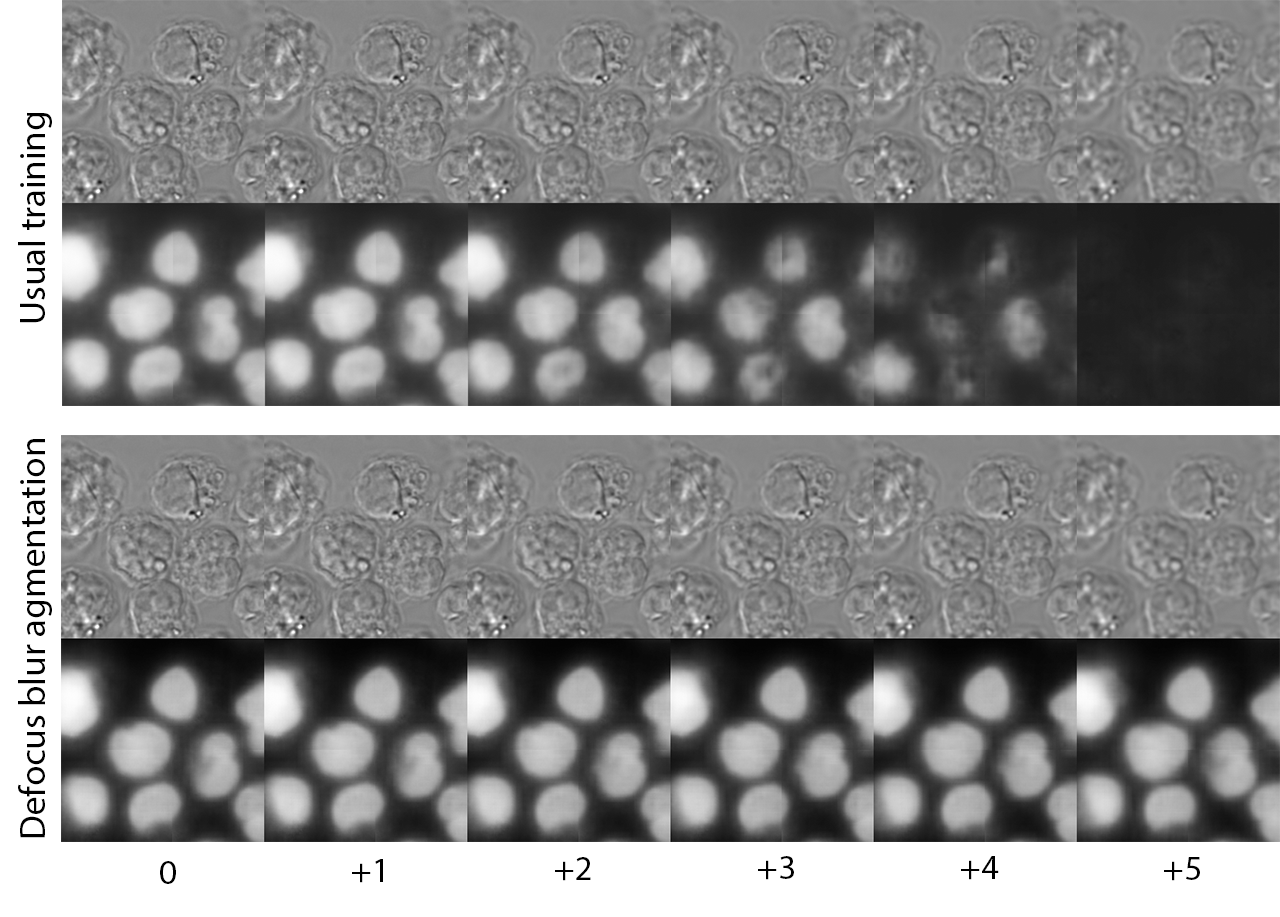
\includegraphics[width=0.4\linewidth]{bilder/stability/augments-help.png}
		\caption[Using corruptions as augmentations to improve predictions: artificial defocus blur example]%
        {Using corruptions as augmentations to improve predictions: artificial defocus blur example}\label{fig:augments-help}
	\end{center}
\end{figure}

Using artificial corruptions in training augmentations positively influences the predictions on the images with real microscopy settings corruptions. See the comparison of the predictions of the model trained with (b) and without (a) artificial corruptions in augmentations on the corrupted dataset with real microscopy settings corruptions in Figure \ref{fig:augments-help-real}. For all types of the corruptions presented there it is clear that predictions the model trained with artificial corruptions are better. The "shine" artifact around the cells is much less pronounced and for wrong exposure and fixation times corruptions there are more details inside the nuclei. In defocus blur corruption case it seems that the outlines of the nuclei are better preserved, however the intensities are still not captured for some of the cells at all. This shows that using corruptions as augmentations can strongly help the model to imrpove predictions for the corrupted images during inference. For the future research it is recommended to add real corruptions data along with the staining into the dataset.
\begin{figure}[htb]
	\begin{center}
		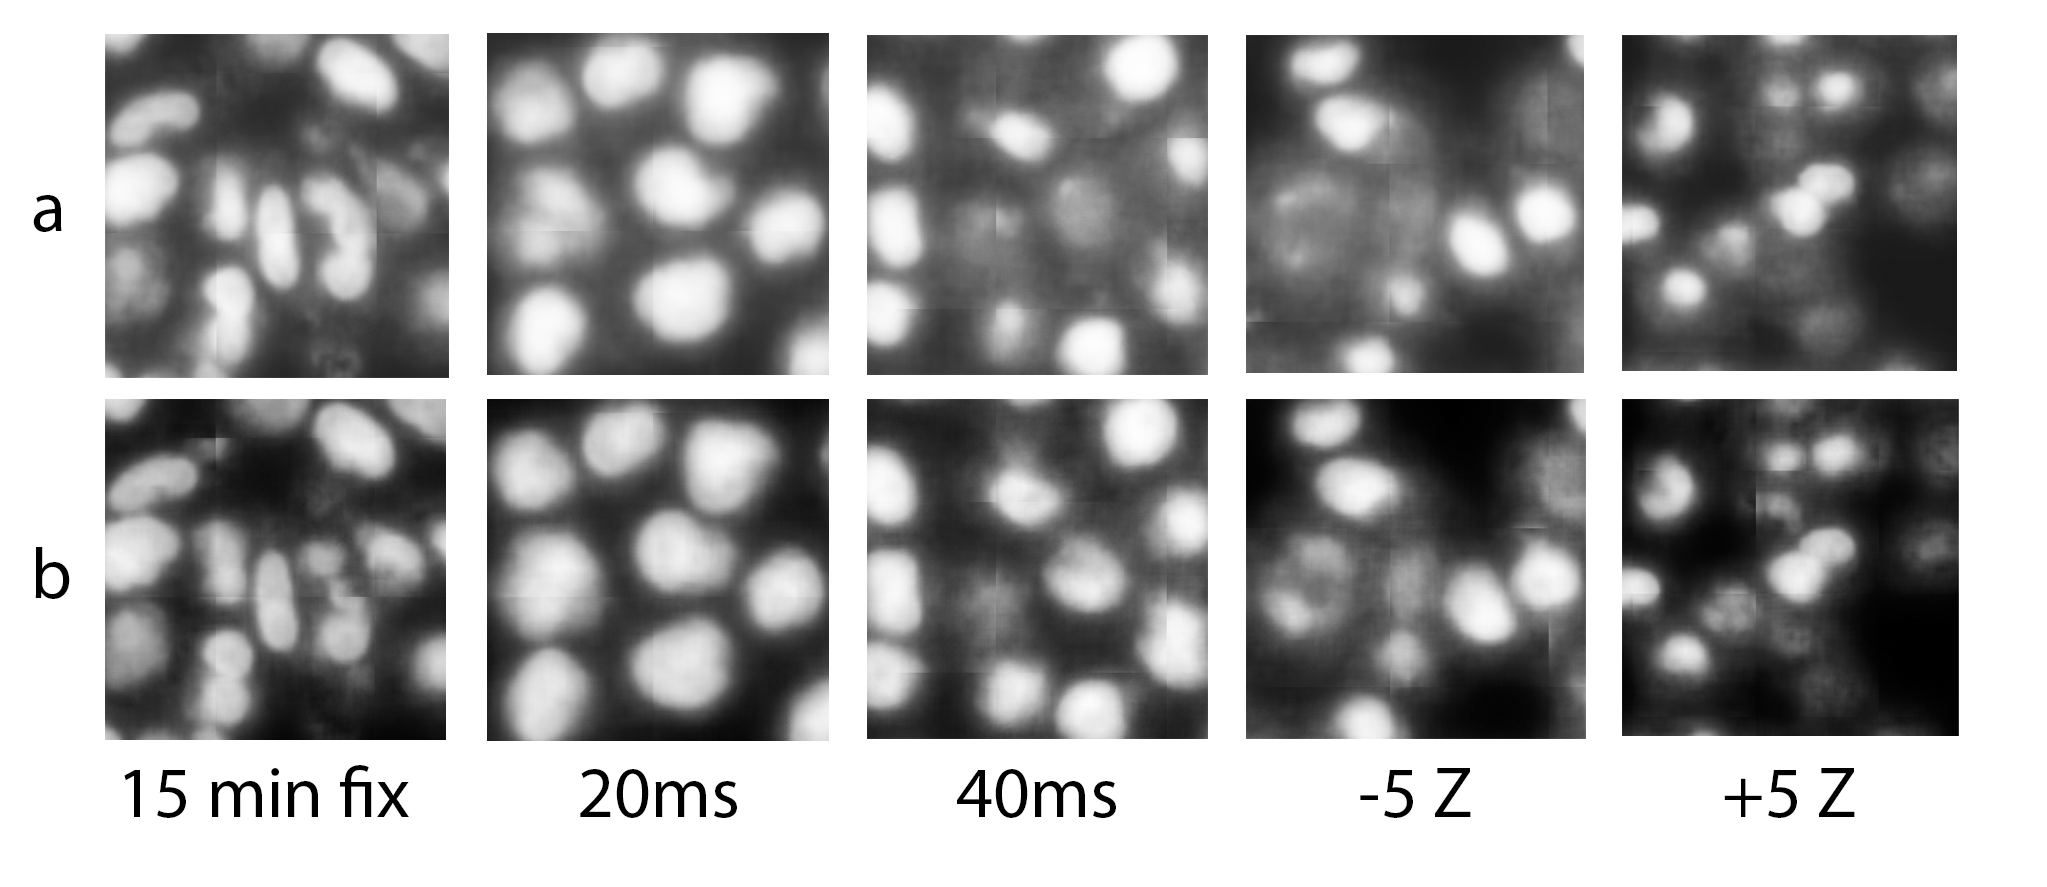
\includegraphics[width=0.6\linewidth]{bilder/stability/augments-help-real.png}
		\caption[Using corruptions as augmentations to improve predictions: real corruptions example]%
        {Using corruptions as augmentations to improve predictions: real corruptions example. (a) --- model trained without artificial corruprions as augmentations; (b) --- model trained with artificial corruptions as augmentations}\label{fig:augments-help-real}
	\end{center}
\end{figure}

\subsubsection{Influence of corruptions on metrics for practical biological evaluation}
Additionally, since for artificial corruptions the ground truth data from staining is present, the difference in biological metrics for models with and without augmentations was measured (see Table \ref{table:nuclei-corruptions-downstream-metrics-coefficients}), more specifically Spearman rank correlarion coefficients were compared. The calculation of biological metrics remained the same except for the thresholding algorithm that was switched to a global one due to the time limit. This results in the wrong segmentation of some of the ground ground truth images due to the illumination inconsistences Therefore Spearman rank correlation coefficient is more repesentative here since it is more stable towards the outliers. The rest of the postprocessing procedure has remained the same apart from the application of artificial corruptions on the input data.

\begin{table}[htb]
    \centering
    \caption{Correlation coefficients for practical biological evaluation on nuclei}
            \begin{tabular}{|c|c|c|c|c|}\hline
                Contrast level&Number of nuclei&Total intensity&Mean intensity&Area\\\hline\hline
                +1&0.934&0.825&0.826&0.898\\\hline
                +2&0.932&0.820&0.819&0.899\\\hline
                +3&0.934&0.799&0.822&0.890\\\hline
                +4&0.804&0.439&0.671&0.540\\\hline
                +5&0.394&0.351&0.383&0.313\\\hline \hline
				Defocus blur level&Number of nuclei&Total intensity&Mean intensity&Area\\\hline\hline
                +1&0.934&0.832&0.827&0.905\\\hline 
                +2&0.929&0.800&0.820&0.890\\\hline
                +3&0.934&0.756&0.8210&0.871\\\hline
                +4&0.838&0.361&0.666&0.501\\\hline
                +5&-0.072&-0.233&-0.231&0.07\\\hline
            \end{tabular}
        \label{table:nuclei-corruptions-downstream-metrics-coefficients}
\end{table} 

One can observe from the table above that the metrics degrade quite fast starting from the severity level $3$. Which aligns well with the visual evaluation of corruptions in Figure \ref{fig:artificial-corruptions} where level $3$ of contrast and defocus blur corruptions affect the intensities and level $4$ affects the whole nuclei outline. Biological metrics confirm that the most affected metrics are the total and mean intensities, whereas the number of organelles seems to be the most stable metric until the very last severity level where the predictions turn almost completely black. Although these metrics are much more representative than PCC or MSE loss they also they their own downsides. For example, severity level $4$ produces not reliable predictions, however correlation coefficient of mean intensity is not completely low --- $0.67$. Therefore it is important to assess predictions quality visually and keep in mind that biological metrics should be ideally quite high.